\documentclass[11pt,a4paper]{article}
\usepackage[margin=1in]{geometry}
\usepackage{amsmath,amssymb}
\usepackage{graphicx}
\usepackage{enumitem}
\usepackage{tcolorbox}
\usepackage{array}
\usepackage{multirow}
\usepackage{tikz}
\usetikzlibrary{positioning,arrows.meta,shapes}

% Custom commands
\newcommand{\highlight}[1]{\textbf{#1}}

% Box for exercises
\newtcolorbox{exercise}[1][]{
    colback=blue!5!white,
    colframe=blue!75!black,
    title=#1,
    fonttitle=\bfseries
}

\newtcolorbox{discovery}[1][]{
    colback=yellow!5!white,
    colframe=orange!75!black,
    title=Discovery Moment,
    fonttitle=\bfseries
}

\newtcolorbox{think}[1][]{
    colback=green!5!white,
    colframe=green!75!black,
    title=Think About It,
    fonttitle=\bfseries
}

\title{\textbf{Week 2: Teaching Computers to Understand Word Relationships}\\
\large Discovering How Machines Learn Language\\
\large Pre-Lab Exercise (No Programming Required)}
\author{NLP Course 2025 - Student Version}
\date{}

\begin{document}
\maketitle

\noindent\textbf{Time:} 30-40 minutes\\
\textbf{Objective:} Discover three fundamental ways computers can learn word meanings from text.

\section*{Part 1: How Words Keep Company (8 minutes)}

\begin{exercise}[Word Prediction Game]
\textbf{Task 1: Fill in the blanks with the most likely word:}
\begin{enumerate}[label=\alph*)]
    \item The cat sat on the \rule{3cm}{0.4pt}
    \item I drink \rule{3cm}{0.4pt} every morning
    \item The \rule{3cm}{0.4pt} barked loudly at the mailman
    \item She wore a beautiful \rule{3cm}{0.4pt} to the wedding
\end{enumerate}

\textbf{Task 2: Reflection}
\begin{enumerate}
    \item How did you know what words to fill in? What clues did you use?
    
    \vspace{2cm}
    
    \item List the words that helped you guess the answer for (a):
    
    Helper words: \rule{8cm}{0.4pt}
    
    \item \textbf{Important Discovery:} You used the surrounding words to predict the missing word. 
    
    In your own words, explain why surrounding words help:
    
    \vspace{2cm}
\end{enumerate}
\end{exercise}

\begin{think}
If humans can guess words from their surroundings, can we teach computers to do the same?
\end{think}

\section*{Part 2: Two Ways to Learn Words (10 minutes)}

\begin{exercise}[Method A: Many Words Predict One]
Imagine you're teaching a computer to fill in blanks like you just did.

\textbf{Scenario:} ``The quick brown \underline{\hspace{2cm}} jumps over''

\textbf{Task 1: Design the Learning}
\begin{enumerate}
    \item What information would you give the computer as INPUT?
    
    INPUT: \rule{8cm}{0.4pt}
    
    \item What should the computer learn to OUTPUT?
    
    OUTPUT: \rule{8cm}{0.4pt}
    
    \item Draw how this works (use arrows):
    \begin{center}
    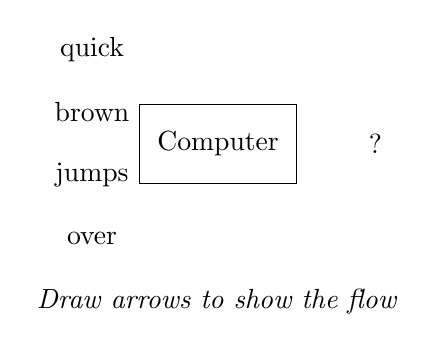
\begin{tikzpicture}[scale=0.8]
        \node at (-2, 1.5) {quick};
        \node at (-2, 0.5) {brown};
        \node at (-2, -0.5) {jumps};
        \node at (-2, -1.5) {over};
        
        \node[draw, rectangle, minimum width=2cm, minimum height=1cm] at (0, 0) {Computer};
        
        \node at (2.5, 0) {?};
        
        \node at (0, -2.5) {\textit{Draw arrows to show the flow}};
    \end{tikzpicture}
    \end{center}
\end{enumerate}

\textbf{Task 2: Practice Examples}

Using Method A (surrounding words → missing word), predict:
\begin{enumerate}
    \item [dog, walked, the, park] → \rule{3cm}{0.4pt}
    \item [ate, pizza, for, lunch] → \rule{3cm}{0.4pt}
\end{enumerate}
\end{exercise}

\begin{discovery}
Congratulations! You've just invented an approach that computer scientists call ``CBOW'' (Continuous Bag of Words). It uses context words to predict a center word - just like you did!
\end{discovery}

\begin{exercise}[Method B: One Word Predicts Many]
Now let's flip it around!

\textbf{Scenario:} Given the word ``coffee'', predict what words often appear near it.

\textbf{Task 1: Word Association}
\begin{enumerate}
    \item Given ``coffee'', list 4 words that often appear nearby:
    \begin{itemize}
        \item \rule{3cm}{0.4pt}
        \item \rule{3cm}{0.4pt}
        \item \rule{3cm}{0.4pt}
        \item \rule{3cm}{0.4pt}
    \end{itemize}
    
    \item This is the OPPOSITE of Method A. Complete:
    \begin{itemize}
        \item Method A: Many words → \rule{3cm}{0.4pt}
        \item Method B: One word → \rule{3cm}{0.4pt}
    \end{itemize}
    
    \item Which method creates MORE training examples from one sentence? Why?
    
    \vspace{2cm}
\end{enumerate}
\end{exercise}

\begin{discovery}
You've discovered ``Skip-gram''! It takes one word and predicts the surrounding context - the reverse of CBOW.
\end{discovery}

\section*{Part 3: Making It Faster - A Clever Trick (10 minutes)}

\begin{exercise}[The Speed Problem]
\textbf{The Challenge:} English has about 50,000 common words. Every time the computer learns, should it:
\begin{itemize}
    \item Option A: Check all 50,000 words to find the right one?
    \item Option B: Check just 5-10 words?
\end{itemize}

Obviously, Option B is faster! But how can we do this?

\textbf{Task 1: Real or Fake?}

Instead of finding THE right word out of 50,000, let's play a simpler game:

Given word pairs, decide if they're REAL (actually appear together) or FAKE (random pairing):

\begin{center}
\begin{tabular}{|l|l|c|}
\hline
\textbf{Word 1} & \textbf{Word 2} & \textbf{Real or Fake?} \\
\hline
coffee & drink & \rule{2cm}{0.4pt} \\
\hline
coffee & elephant & \rule{2cm}{0.4pt} \\
\hline
dog & barked & \rule{2cm}{0.4pt} \\
\hline
dog & galaxy & \rule{2cm}{0.4pt} \\
\hline
queen & king & \rule{2cm}{0.4pt} \\
\hline
queen & bicycle & \rule{2cm}{0.4pt} \\
\hline
\end{tabular}
\end{center}

\textbf{Task 2: Understanding the Trick}
\begin{enumerate}
    \item Instead of asking ``Which of 50,000 words is correct?'', we now ask:
    
    New question: \rule{8cm}{0.4pt}
    
    \item For each real pair, how many fake pairs should we create for good learning?
    
    \rule{2cm}{0.4pt} fake pairs
    
    \item If we use 5 fake pairs + 1 real pair, we only update 6 words instead of 50,000.
    
    What's the speedup? \rule{3cm}{0.4pt} times faster!
\end{enumerate}
\end{exercise}

\begin{discovery}
This clever trick is called ``Negative Sampling''! The real pairs are ``positive samples'' and the fake pairs are ``negative samples''. It makes training about 8,000 times faster!
\end{discovery}

\section*{Part 4: Comparing Your Discoveries (7 minutes)}

\begin{exercise}[Putting It All Together]
Now that you understand all three approaches, let's compare them:

\begin{center}
\begin{tabular}{|l|p{3.5cm}|p{3.5cm}|p{3.5cm}|}
\hline
\textbf{Aspect} & \textbf{Method A} & \textbf{Method B} & \textbf{The Speed Trick} \\
& \textbf{(CBOW)} & \textbf{(Skip-gram)} & \textbf{(Negative Sampling)} \\
\hline\hline
What goes IN? & Multiple context & & \\
(Input) & words & & \\
\hline
How does it & Combine all & & \\
work? & context words & & \\
(Method) & & & \\
\hline
What comes & & Multiple context & \\
OUT? & & words & \\
(Output) & & & \\
\hline
Example & [cat, sat, the] & & (coffee, drink) \\
& → on & & → Real \\
\hline
Best for & Common words & & Making training \\
& & & faster \\
\hline
\end{tabular}
\end{center}

\textbf{Critical Thinking Questions:}
\begin{enumerate}
    \item Why might Method B (Skip-gram) work better for rare words than Method A (CBOW)?
    
    \textit{Hint: Think about how many training examples each method creates.}
    
    \vspace{2cm}
    
    \item The Speed Trick changes the question from ``which word?'' to ``real or fake?'' 
    
    Why is this simpler for a computer?
    
    \vspace{2cm}
    
    \item If you wanted to find words similar to ``doctor'', which method would you choose? Why?
    
    \vspace{2cm}
\end{enumerate}
\end{exercise}

\section*{Part 5: Real-World Impact (5 minutes)}

\begin{exercise}[Reflection]
\textbf{You've just discovered three fundamental techniques that power modern AI language models!}

\begin{enumerate}
    \item These techniques help computers understand that ``king'' and ``queen'' are related. 
    
    How do you think the computer learns this relationship?
    
    \vspace{2cm}
    
    \item Word prediction is used in your phone's keyboard. 
    
    Which method (A or B) do you think works better for predicting your next word? Why?
    
    \vspace{2cm}
    
    \item Before these methods, computers needed humans to manually teach every word relationship.
    
    What's the advantage of learning from context automatically?
    
    \vspace{2cm}
\end{enumerate}
\end{exercise}

\vspace{1cm}
\noindent\rule{\textwidth}{0.4pt}
\begin{center}
\textbf{Summary}: You discovered three key concepts today:\\
\textbf{CBOW} (many→one), \textbf{Skip-gram} (one→many), and \textbf{Negative Sampling} (real vs fake).\\
These are the foundations of modern language AI!
\end{center}

\end{document}